% Compile with: pdflatex (or lualatex/xelatex if you prefer)
% Figures are in the folder slides_figures/ (extracted from the executed notebook).
% Not compiled on the machine that wrote it (no LaTeX installed there): compile once and fix any warning.
\documentclass[aspectratio=169]{beamer}

% -------------------- THEME (RED BASE) --------------------
\usetheme{Madrid}
\usecolortheme{default}

\definecolor{BaseRed}{RGB}{170,0,0}
\setbeamercolor{structure}{fg=BaseRed}
\setbeamercolor{frametitle}{fg=white,bg=BaseRed}
\setbeamercolor{title}{fg=white,bg=BaseRed}
\setbeamercolor{block title}{fg=white,bg=BaseRed}
\setbeamercolor{block body}{bg=BaseRed!5}
\setbeamercolor{alerted text}{fg=BaseRed}

\setbeamertemplate{navigation symbols}{}
\setbeamertemplate{footline}[frame number]

% -------------------- PACKAGES --------------------
\usepackage[T1]{fontenc}
\usepackage{graphicx}
\usepackage{amsmath,amssymb,amsfonts}
\usepackage{booktabs}
\usepackage{hyperref}
\usepackage{algorithm}
\usepackage[noend]{algpseudocode}

\graphicspath{{slides_figures/}}

\hypersetup{
  colorlinks=true,
  linkcolor=BaseRed,
  urlcolor=BaseRed,
  citecolor=BaseRed
}
\urlstyle{rm}

% -------------------- METADATA --------------------
\title[CartPole: OG vs NN vs Nuclei]{CartPole: OG vs NN vs Nuclei}
\subtitle{From hand-written rules to a ReLU Q-network, patience, and more CPU cores}
\author[Authors]{[Author name] \and Bryan [surname]}
\institute[Intelligent Agents]{Intelligent Agents\\RL101 -- CartPole activity\\\texttt{[email]}}
\date{\today}

\begin{document}

% -------------------- TITLE --------------------
\begin{frame}
  \titlepage
\end{frame}

% -------------------- OUTLINE --------------------
\begin{frame}{Outline}
\tableofcontents
\end{frame}

% =========================================================
\section{Introduction}

\begin{frame}{Motivation}
\begin{itemize}
  \item \textbf{CartPole-v1}: push a cart left or right to keep a pole upright; reward $+1$ per step, so the \alert{return is the number of steps survived}, capped at 500.
  \item The original activity (\textbf{OG}) solves it with two-line \emph{hand-written rules} and ends with a bridge to DQN.
  \item Two extensions were built on top of it:
  \begin{itemize}
    \item \textbf{NN}: replace the rule by a learned Q-network (ReLU), and make its training trustworthy (patience, best checkpoint, CPU vs GPU time).
    \item \textbf{Nuclei} (Bryan): run the DQN lab's experiments on \alert{more CPU cores}.
  \end{itemize}
  \item Main question: what does each idea buy, in \alert{quality} and in \alert{time}?
\end{itemize}
\end{frame}

\begin{frame}{Objective}
\begin{block}{Main objective}
Integrate the two experiments in one notebook, keep them separate, and compare \textbf{OG vs NN vs Nuclei} on the same seeds, with the same protocol, measuring quality and wall-clock time.
\end{block}

\begin{itemize}
  \item Understand why the OG rules work (and when they fail) before learning anything.
  \item NN: obtain a stable learned policy; show what patience, a grace period and checkpoint restore each contribute.
  \item Nuclei: measure what more cores buy, and check that results do not change.
  \item Report honestly: small samples, selection effects, what was not run.
\end{itemize}
\end{frame}

\begin{frame}{Three experiments, one notebook}
\small
\begin{table}
\centering
\begin{tabular}{p{1.9cm}p{3.1cm}p{4.9cm}p{4.3cm}}
\toprule
\textbf{Section} & \textbf{Whose} & \textbf{What} & \textbf{How it is integrated}\\
\midrule
OG & course activity & state, actions, human play, rule-based policies, ``break the environment'' & 22 cells copied \emph{verbatim}, stored outputs kept\\
NN & notebook author & ReLU DQN, double DQN + soft target, patience with grace period, CPU vs GPU & new cells, names prefixed \texttt{NN}\\
Nuclei & Bryan & DQN lab; \texttt{joblib} \texttt{run\_configs} on 8 cores & 52 cells \emph{verbatim}; two marked measurements added\\
Comparison & both & OG vs NN vs Nuclei, quality and time & new cells; time ledger per cell\\
\bottomrule
\end{tabular}
\end{table}
\end{frame}

% =========================================================
\section{Background / Theory}

\begin{frame}{CartPole as a Markov decision process}
\begin{itemize}
  \item \textbf{State} $s=(x,\dot x,\theta,\dot\theta)$: cart position, cart velocity, pole angle, pole angular velocity.
  \item \textbf{Actions}: $0$ = push left, $1$ = push right (fixed force 10 N); \textbf{reward} $+1$ per step; time step $\tau=0.02$ s.
  \item \alert{Terminated}: $|\theta|>0.2095$ rad ($12^\circ$) or $|x|>2.4$ m (a true failure). \alert{Truncated}: 500 steps (v0: 200), just the clock.
  \item \textbf{Return} $G=\sum_t r_t$ = steps survived; the goal is a policy $\pi(s)\to a$ maximizing it.
\end{itemize}
\begin{block}{Why the distinction matters}
A time-limit cut is not a failure: the DQN target must bootstrap through \emph{truncation} and stop only at \emph{termination}.
\end{block}
\end{frame}

\begin{frame}{Physics and the rule-based controller (OG)}
\begin{block}{Equations of motion (gymnasium source, Euler integration)}
\[
\ddot\theta=\frac{g\sin\theta-\cos\theta\,\dfrac{F+m_p l\dot\theta^2\sin\theta}{M}}{l\left(\frac43-\dfrac{m_p\cos^2\theta}{M}\right)},\qquad
\ddot\theta\approx 15.8\,\theta-14.6\,u,\; u=\pm1
\]
\end{block}
\begin{itemize}
  \item Checked on the printed numbers: predicted $\Delta\dot\theta=13.9\cdot0.02=0.278$; observed $0.2295-(-0.0483)=0.278$.
  \item Gravity is unstable ($15.8\,\theta$), but one push ($14.6$) beats gravity at the failure angle ($3.3$): only the \emph{timing} of the switch matters.
  \item Rule: push right iff $s=\theta+K\dot\theta\ge0$. On $s=0$: $\theta(t)=\theta_0e^{-t/K}$ (PD / sliding-mode control).
  \item $K\to0$ is the angle-only rule, $K\to\infty$ the angular-velocity-only rule.
\end{itemize}
\end{frame}

\begin{frame}{From a Q-table to a Q-network}
\begin{block}{Bellman target and DQN loss}
\[
y=r+\gamma\,(1-\text{terminated})\,\max_{a'}Q_{\bar\theta}(s',a'),\qquad
L(\theta)=\mathbb{E}\big[\mathrm{Huber}\big(y-Q_\theta(s,a)\big)\big]
\]
\end{block}
\begin{itemize}
  \item A table needs a finite state set: 10 bins per variable already give $10^4\cdot2=20{,}000$ entries and grow as $N^4$.
  \item The network $Q_\theta:\mathbb{R}^4\to\mathbb{R}^2$ is $4\to128\to128\to2$ with \textbf{ReLU} after both hidden layers and a \emph{linear} output ($17{,}410$ parameters); the policy is $\arg\max_a Q_\theta(s,a)$.
  \item Replay buffer (20,000 transitions, batch 64) breaks the correlation of consecutive steps; $\epsilon$-greedy explores ($1.0\to0.05$ over 5,000 steps).
  \item The \alert{loss is a surrogate}: the success metric is the greedy episode return.
\end{itemize}
\end{frame}

\begin{frame}{Stabilisers: double DQN and soft target}
\begin{block}{Double DQN (choose with the online net, score with the target net)}
\[
y=r+\gamma\,(1-\text{terminated})\;Q_{\bar\theta}\!\big(s',\arg\max_{a'}Q_\theta(s',a')\big)
\]
\end{block}
\begin{block}{Soft (Polyak) target update, every step}
\[
\bar\theta\leftarrow(1-\tau)\,\bar\theta+\tau\,\theta,\qquad \tau=0.02
\]
\end{block}
\begin{itemize}
  \item Plain DQN: hard copy every 300 steps and a plain $\max$ (the lab default).
  \item Diagnosis of the plain run (N0): max-Q keeps growing (about 4 $\to$ 30--34 in 12,000 steps) while the greedy return swings between about 100 and 500.
  \item $\tau$ has a cliff: $\tau=0.005$--$0.02$ worked, $\tau=0.05$ collapsed on the development seeds.
\end{itemize}
\end{frame}

\begin{frame}{Patience, grace period and best checkpoint}
\scriptsize
\begin{algorithm}[H]
\caption{Patience with a grace period (validation every 1,000 steps)}
\begin{algorithmic}[1]
\State \textbf{Input:} patience $P$, grace step $g$, $\Delta=1$; $best\leftarrow-\infty$, $bad\leftarrow0$
\For{each validation at step $t$}
  \State $score\leftarrow$ greedy return on 10 fixed validation episodes
  \If{$score>best+\Delta$}
    \State $best\leftarrow score$; save a copy of the weights; $bad\leftarrow0$
  \ElsIf{$t\ge g$}
    \State $bad\leftarrow bad+1$
  \EndIf
  \If{$bad\ge P$} \textbf{stop} \EndIf
\EndFor
\State \textbf{Output:} the \emph{best} saved weights (not the last ones)
\end{algorithmic}
\end{algorithm}
\normalsize
\begin{itemize}
  \item \alert{Restoring the best} and \alert{stopping early} are different effects; the grace period keeps an early plateau from stopping training.
\end{itemize}
\end{frame}

\begin{frame}{Nuclei: more cores}
\begin{itemize}
  \item Bryan's \texttt{run\_configs} sends each (configuration, seed) training to a worker with \texttt{joblib.Parallel(n\_jobs=8)}.
  \item The trainings are independent and each \texttt{train()} seeds itself, so \alert{parallel and sequential must give the same result}; his comment claims it, we test it.
  \item Ideal speed-up with $n$ workers and a parallel fraction $p$ (Amdahl):
\end{itemize}
\begin{block}{Speed-up bound}
\[
S(n)\le\frac{1}{(1-p)+p/n},\qquad \text{here also capped by } \lceil \#\text{trainings}/n\rceil \text{ rounds}
\]
\end{block}
\begin{itemize}
  \item The laptop has 8 logical but 4 physical cores, and every worker pays process start-up and a \texttt{torch} import.
\end{itemize}
\end{frame}

% =========================================================
\section{Implementation}

\begin{frame}{Implementation Details}
\begin{itemize}
  \item Python, \texttt{gymnasium} 1.3, \texttt{torch} 2.11 (CUDA 12.8), \texttt{joblib}; one Jupyter kernel, 8 logical cores, RTX 4050 Laptop GPU.
  \item \textbf{OG}: 22 original cells copied verbatim; \texttt{evaluate\_policy} is reused by every later section.
  \item \textbf{NN}: \texttt{NNQNetwork}, \texttt{NNReplayBuffer}, \texttt{PatienceStopper}, \texttt{train\_nn} (options: \texttt{double}, \texttt{tau}, \texttt{dropout}, \texttt{patience}, \texttt{grace}, \texttt{device}).
  \item \textbf{Nuclei}: 52 of Bryan's cells verbatim (his \texttt{.long()} fix for Windows included); heaviest cells shipped unexecuted.
  \item \textbf{Comparison}: a hook records the network that Bryan's unchanged \texttt{train()} builds, so OG DQN weights can be scored.
  \item Every cell is timed from the notebook's own timestamps; the notebook is saved after every cell.
\end{itemize}
\end{frame}

\begin{frame}{Agent settings (NN)}
\small
\begin{table}
\centering
\begin{tabular}{ll}
\toprule
\textbf{Item} & \textbf{Value}\\
\midrule
Network & $4\to128\to128\to2$, ReLU, linear output, 17,410 parameters\\
Optimiser / loss & Adam, lr $5\cdot10^{-4}$; Huber loss; gradient clip 10\\
Discount / batch / buffer & $\gamma=0.99$; 64; 20,000 transitions; learning starts at 1,000\\
Exploration & $\epsilon$: $1.0\to0.05$ over 5,000 steps\\
Target & plain: hard copy every 300 steps; recipe: double DQN + soft $\tau=0.02$\\
Patience & validation every 1,000 steps on 10 episodes; grace 15,000; $P=10$; $\Delta=1$\\
Dropout (ablation) & 0.1 after both hidden layers; off when acting, validating, and in the target net\\
\bottomrule
\end{tabular}
\end{table}
\end{frame}

\begin{frame}{Seeds and data roles}
\begin{itemize}
  \item No dataset: episodes come from the simulator; what must be controlled is \alert{which seeds play which role}.
\end{itemize}
\small
\begin{table}
\centering
\begin{tabular}{lll}
\toprule
\textbf{Role} & \textbf{Seeds} & \textbf{Used for}\\
\midrule
Training starts & $1000+$ training seed & learning only ($\epsilon$-greedy, noisy)\\
Validation & 10,000--10,009 & patience decisions and checkpoint choice\\
Development & train 100--102, 200--204; test 20,000--20,049 & choosing the recipe ($\tau$, double, ...)\\
First final & train 300--304; test 30,000--30,049 & showed why patience needs a grace period\\
\textbf{Final} & \textbf{train 400--404; test 40,000--40,049} & \textbf{nothing was tuned on these}\\
\bottomrule
\end{tabular}
\end{table}
\end{frame}

% =========================================================
\section{Analysis}

\begin{frame}{Methodology}
\begin{itemize}
  \item \textbf{One change at a time}: plain $\to$ recipe $\to$ recipe + grace patience (and last weights vs restored best from the same run).
  \item \textbf{Selection vs final}: the recipe was chosen on development seeds; the grace period after seeing seeds 300--304; the headline numbers use seeds 400--404 that nobody had looked at.
  \item \textbf{Determinism}: training is seeded and validation draws no random numbers, so patience runs follow the full run until they stop, and two independent runs of the same design gave identical tables.
  \item \textbf{Time}: \texttt{time.perf\_counter()} around whole batches; \texttt{torch.cuda.synchronize()} before reading the clock on the GPU; contended times are labelled as such.
  \item \textbf{Metric}: greedy return on 50 fresh episodes, per training seed, with the failure mode where useful.
\end{itemize}
\end{frame}

\begin{frame}{Time Complexity}
Let $P=17{,}410$ be the number of parameters, $B=64$ the batch, $T$ the number of environment steps.

\begin{block}{Per-operation complexity}
\begin{itemize}
  \item Acting: one forward pass, $O(P)$ ($\approx 3.5\cdot10^4$ FLOPs).
  \item Replay add / sample: $O(1)$ / $O(B)$.
  \item Update (double DQN): forward on $s$, backward, forward on $s'$ with both nets, $\approx10\,B\,P\approx1.1\cdot10^7$ FLOPs; soft target $O(P)$.
  \item Validation: $V$ episodes $\times$ up to 500 steps $\times\,O(P)$.
\end{itemize}
\end{block}

\begin{block}{Total complexity}
\[
T_{\text{train}}=O(T\cdot B\cdot P)\quad\Rightarrow\quad\text{patience reduces }T\text{ (24{,}200 instead of 30{,}000 steps)}
\]
\end{block}
\small Measured: one update takes 2.8 ms on one CPU thread, far from the arithmetic bound, so Python/PyTorch call overhead dominates (not profiled).
\end{frame}

\begin{frame}{Space Complexity}
\begin{block}{Space requirements}
\begin{itemize}
  \item Replay buffer: $20{,}000\times(4+4)$ floats $+$ action, reward, flag $\approx48$ B each $\approx 0.96$ MB: $O(N_{\text{buf}})$.
  \item Parameters: $17{,}410\times4$ B $\approx70$ kB; online, target, gradients and two Adam moments $\approx0.35$ MB: $O(P)$.
  \item Tabular alternative: $N^{4}\cdot 2$ entries (20,000 for 10 bins), exponential in the number of variables.
\end{itemize}
\end{block}

\begin{block}{Overall space complexity}
\[
S=O(N_{\text{buf}}+P)\ \text{per training; with } n \text{ workers } n\times\text{ that, plus one Python/torch runtime each}
\]
\end{block}
\end{frame}

% =========================================================
\section{Experimental Results}

\begin{frame}{Experimental Setup}
\begin{itemize}
  \item All runs: one machine, CPU unless stated; 30,000-step budget for every DQN.
  \item \textbf{OG}: 4 rules $\times$ 20 episodes (seeds 0--19), plus earlier checks on 200 unseen seeds.
  \item \textbf{NN}: development sweeps (3--5 seeds, 12 configurations), story on seeds 300--304, \alert{live final run: 15 trainings, seeds 400--404}.
  \item \textbf{CPU/GPU}: 5,000-step runs on three devices, per-operation timing, size sweep.
  \item \textbf{Nuclei}: Bryan's \texttt{run\_configs}, 6 trainings $\times$ 6,000 steps at 1/2/4/8 workers.
  \item \textbf{Comparison}: OG DQN and NN, 5 seeds $\times$ 30,000 steps on 8 cores; sequential time measured on one training and scaled (labelled estimate).
  \item \alert{Trimmed to a 60-minute budget}: Bryan's 50,000-step runs and Part 5 runs A--E are shipped unexecuted.
\end{itemize}
\end{frame}

\begin{frame}{Results: OG rules (seeds 0--19)}
\small
\begin{table}
\centering
\begin{tabular}{lccl}
\toprule
\textbf{Policy} & \textbf{Mean $\pm$ std} & \textbf{Ends by} & \textbf{Why}\\
\midrule
random & $24.0\pm8.2$ & pole & ignores the state\\
angle only & $40.9\pm7.4$ & pole, 20/20 & no damping: oscillation grows\\
angular velocity only & $198.7\pm36.3$ & cart, 20/20 & freezes rotation, not tilt: cart runs away\\
angle $+\,K\cdot$ ang. vel., $K=1$ & $491.7\pm36.2$ & 19 time limit, 1 cart & PD / sliding-mode\\
\bottomrule
\end{tabular}
\end{table}
\begin{itemize}
  \item Earlier checks: $K=0.1$--$0.5$ gave $500\pm0$ on seeds 0--19; on 200 unseen seeds $K=1$ lost 30 episodes to the cart ($477.2\pm56.5$) while $K=0.25,0.5$ gave $500\pm0$.
  \item Wider start noise ($\pm0.3$) cut $K=1$ to 163.1; about 31\% of such starts begin outside the $12^\circ$ limit.
\end{itemize}
\end{frame}

\begin{frame}{Results: choosing the recipe (development seeds 200--204)}
\small
\begin{table}
\centering
\begin{tabular}{lcc}
\toprule
\textbf{Configuration} & \textbf{Restored best} & \textbf{Last weights}\\
\midrule
plain DQN (base) & 413.3 & 300.9\\
double + soft $\tau=0.005$ & 498.3 & 454.8\\
double + soft $\tau=0.01$ & 495.5 & 401.3\\
\textbf{double + soft $\tau=0.02$} & \textbf{500.0} & \textbf{500.0}\\
double + soft $\tau=0.02$ + input scaling & 493.8 & 294.6\\
double + soft $\tau=0.05$ & 231.0 & 60.8\\
\bottomrule
\end{tabular}
\end{table}
\begin{itemize}
  \item Not helpful on 3 seeds: lower $\gamma$ (0.95: 375.4; 0.98: 323.0 vs 474.3), 100k buffer, higher learning rate.
  \item \alert{Winner's curse}: about a dozen settings compared on 3--5 seeds; the fresh-seed result is the honest gain.
\end{itemize}
\end{frame}

\begin{frame}{Results: why patience needs a grace period (seeds 300--304)}
\small
\begin{table}
\centering
\begin{tabular}{lcc}
\toprule
\textbf{Run} & \textbf{Test mean} & \textbf{Steps used}\\
\midrule
plain DQN, last weights & 472.0 & 30,000\\
plain DQN, restored best & 500.0 & 30,000\\
recipe, last weights (reported) & 401.8 & 30,000\\
recipe + dropout 0.1, last weights (reported) & 343.8 & 30,000\\
recipe + patience $P=3$, no grace & 256.9 & 7,400\\
recipe + patience $P=5$, no grace & 264.6 & 10,200\\
recipe + patience $P=10$, no grace & 498.9 & 23,600\\
\bottomrule
\end{tabular}
\end{table}
\begin{itemize}
  \item Patience stopped \emph{inside the plateau before the breakthrough}; one recipe seed collapsed to a dead network after scoring 500.
  \item Dropout did not help (single run, weak evidence). These seeds motivated the grace period.
\end{itemize}
\end{frame}

\begin{frame}{Results: final NN experiment (fresh seeds 400--404)}
\small
\begin{table}
\centering
\begin{tabular}{lccc}
\toprule
\textbf{Run} & \textbf{Test by seed} & \textbf{Mean $\pm$ std} & \textbf{Steps}\\
\midrule
plain DQN, last weights & 191/154/180/70/147 & $148.4\pm42.4$ & 30,000\\
plain DQN, restored best & 283/500/500/254/296 & $366.7\pm109.7$ & 30,000\\
recipe, last weights & 9/9/500/500/500 & $303.7\pm240.4$ & 30,000\\
recipe, restored best & 500/408/500/500/493 & $480.3\pm36.0$ & 30,000\\
\textbf{recipe + grace patience} & 500/408/500/500/493 & $\mathbf{480.3\pm36.0}$ & \textbf{24,200}\\
\bottomrule
\end{tabular}
\end{table}
\begin{itemize}
  \item Reproduced \emph{exactly} by an independent run of the same design.
  \item OG rule on its own protocol: $491.7\pm36.2$; the best DQN is close, not above.
\end{itemize}
\end{frame}

\begin{frame}{Figure: the final NN experiment}
\centering
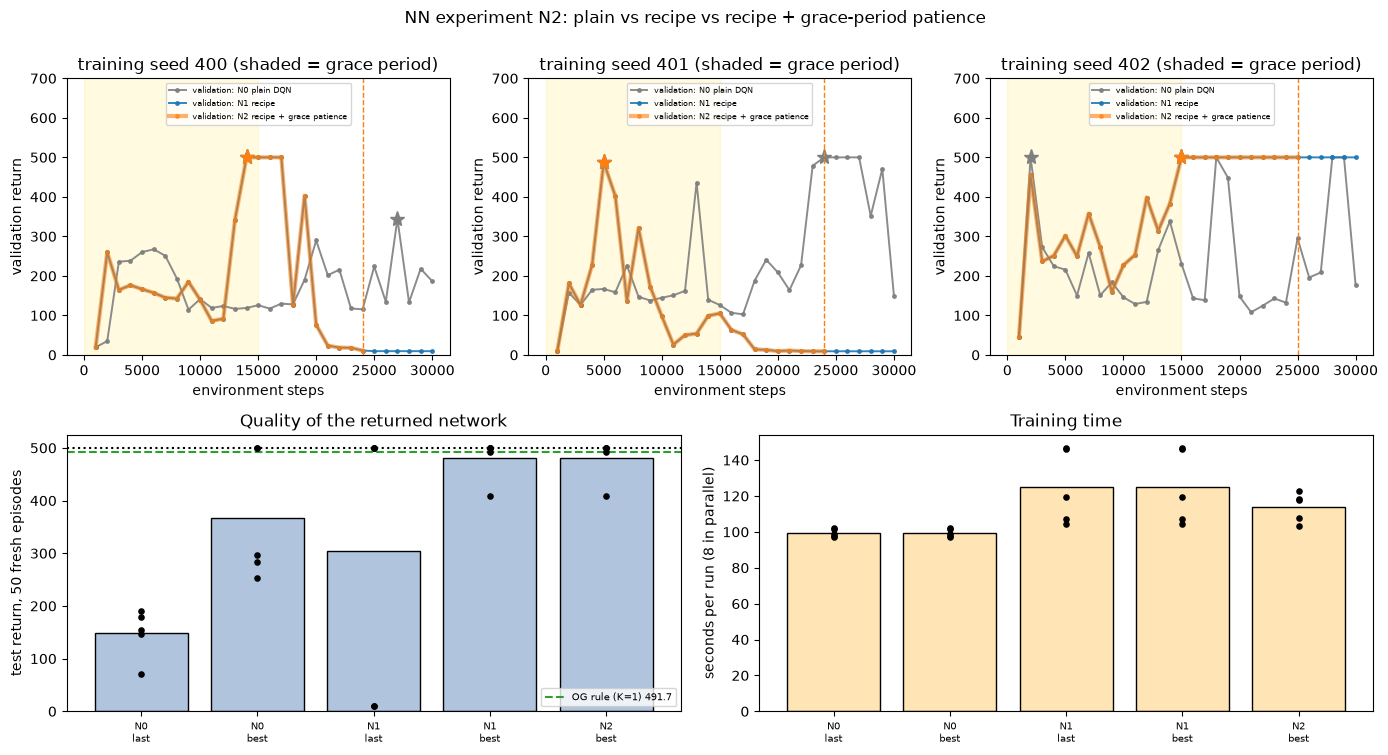
\includegraphics[width=0.78\linewidth]{fig_n2_final.png}

\footnotesize Top: validation curves (shaded = grace period; dashed = stop; $\star$ = best checkpoint). Bottom: test return and training time.
\end{frame}

\begin{frame}{Results Discussion: NN}
\begin{itemize}
  \item \textbf{Largest effect: restoring the best checkpoint} (plain 148 $\to$ 367; recipe 304 $\to$ 480). Two recipe runs ended on a dead network (score 9) after scoring 500.
  \item \textbf{Grace-period patience returns the same networks as training to the end with 19\% fewer steps.} Without the grace period it stopped inside a plateau.
  \item \textbf{The recipe adds about $+113$} over plain DQN once both restore the best (4 seeds better, 1 worse, 1 tied): much less than on the development seeds.
  \item \textbf{Limits}: 5 seeds per arm; grace length and $P$ were designed after seeds 300--304; dropout evidence is a single run; contended per-run seconds are not clean timings.
  \item \textbf{Not claimed}: that the network beats the rule (it does not), or that $\tau=0.02$ is optimal (it sits near a cliff).
\end{itemize}
\end{frame}

\begin{frame}{Results: CPU vs GPU (5,000-step runs)}
\small
\begin{columns}[T,onlytextwidth]
\column{0.5\textwidth}
\begin{table}
\centering
\begin{tabular}{lcc}
\toprule
\textbf{Device} & \textbf{Seconds} & \textbf{Steps/s}\\
\midrule
CPU, 1 thread & 11.7 & 429\\
CPU, 4 threads & 11.8 & 424\\
GPU & 27.0 & 185\\
\bottomrule
\end{tabular}
\end{table}
\begin{table}
\centering
\begin{tabular}{lcc}
\toprule
\textbf{Operation ($\mu$s)} & \textbf{CPU} & \textbf{GPU}\\
\midrule
act & 144 & 722\\
sample + copy & 37 & 418\\
update & 2,785 & 5,152\\
\bottomrule
\end{tabular}
\end{table}
\column{0.5\textwidth}
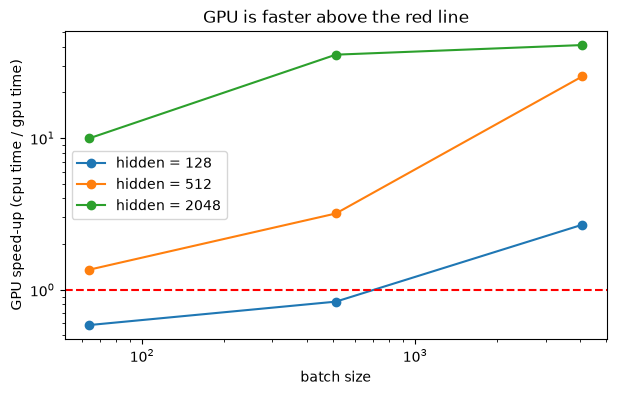
\includegraphics[width=\linewidth]{fig_gpu_speedup.png}
\end{columns}
\begin{itemize}
  \item GPU is 2.3$\times$ \emph{slower} here: each step pays a CPU--GPU round trip and a copy; the network is too small. It wins only for large models or batches (up to 41$\times$ at 2048 units, batch 4096).
\end{itemize}
\end{frame}

\begin{frame}{Results: Nuclei, more cores (Bryan's \texttt{run\_configs})}
\small
\begin{columns}[T,onlytextwidth]
\column{0.5\textwidth}
\begin{table}
\centering
\begin{tabular}{rcccc}
\toprule
\texttt{n\_jobs} & \textbf{s} & \textbf{Speed-up} & \textbf{Eff.} & \textbf{Same?}\\
\midrule
1 & 61.5 & 1.00$\times$ & 100\% & --\\
2 & 30.5 & 2.01$\times$ & 101\% & yes\\
4 & 27.1 & 2.26$\times$ & 57\% & yes\\
8 & 21.4 & 2.88$\times$ & 36\% & yes\\
\bottomrule
\end{tabular}
\end{table}
\column{0.5\textwidth}
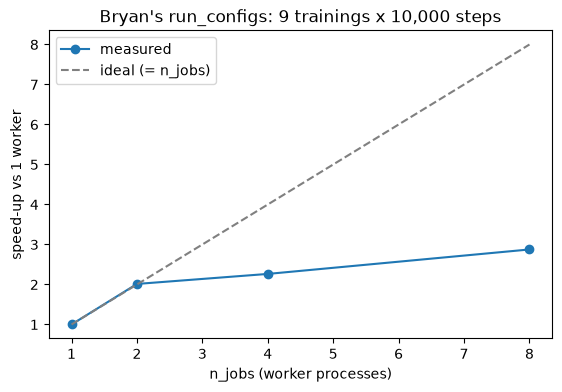
\includegraphics[width=\linewidth]{fig_nuclei_scaling.png}
\end{columns}
\begin{itemize}
  \item 6 trainings $\times$ 6,000 steps. \alert{His claim holds}: curves are bit-for-bit identical at every \texttt{n\_jobs}.
  \item Speed-up is capped by the workload (6 trainings, 4 physical cores) and by process start-up; more workers than physical cores add little.
\end{itemize}
\end{frame}

\begin{frame}{Results: OG vs NN vs Nuclei (seeds 400--404, 50 fresh episodes)}
\scriptsize
\begin{table}
\centering
\begin{tabular}{lcccc}
\toprule
\textbf{Arm} & \textbf{Test by seed} & \textbf{Mean} & \textbf{Steps/run} & \textbf{5 trainings, wall time}\\
\midrule
OG rule, $K=1$ & deterministic & 500.0 & -- & 0.4 s\\
OG DQN, 1 core & 141/161/130/112/148 & 138.2 & 30,000 & $\approx$226 s (\alert{estimate}: $5\times45$ s)\\
\textbf{Nuclei}: OG DQN, 8 cores & identical networks & 138.2 & 30,000 & \textbf{72.9 s} (measured)\\
NN, 1 core & 500/408/500/500/493 & 480.3 & 24,200 & $\approx$250 s (\alert{estimate}: $5\times50$ s)\\
\textbf{NN + Nuclei}, 8 cores & identical networks & 480.3 & 24,200 & \textbf{84.3 s} (measured)\\
\bottomrule
\end{tabular}
\end{table}
\normalsize
\begin{itemize}
  \item \textbf{Quality}: NN $\gg$ OG DQN (480.3 vs 138.2), but neither beats the rule (500.0 on these episodes).
  \item \textbf{Nuclei} changes cost, not quality: 3.1$\times$ (OG DQN) and 3.0$\times$ (NN) faster than the estimated 1-core time; weights bit-identical to sequential.
  \item NN costs 1.11$\times$ the time of the OG DQN on one core (50 s vs 45 s) for 3.5$\times$ the return.
\end{itemize}
\end{frame}

\begin{frame}{Figure: OG vs NN vs Nuclei}
\centering
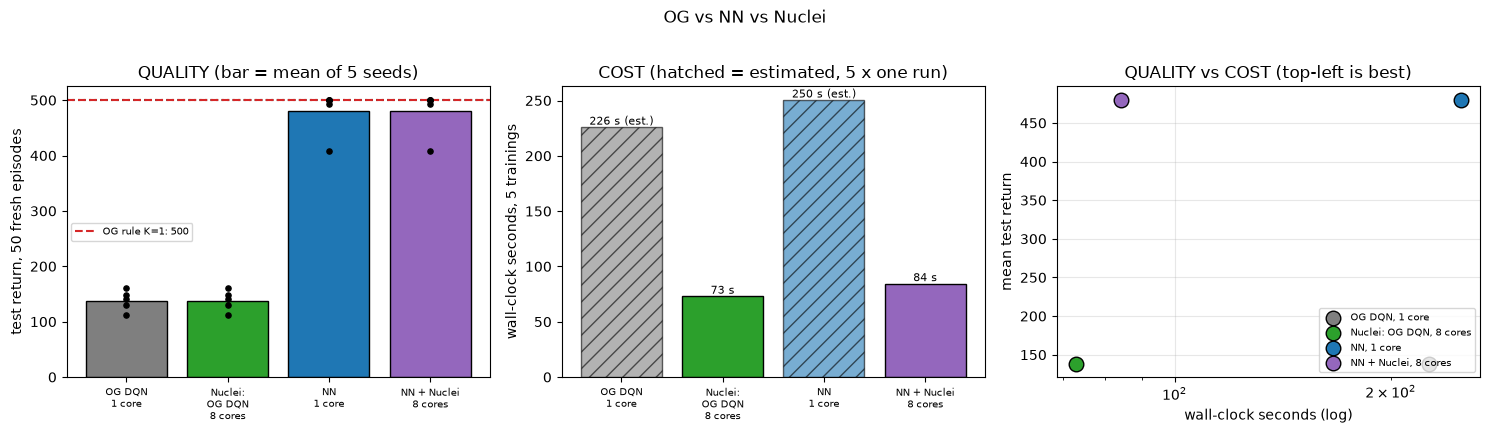
\includegraphics[width=0.95\linewidth]{fig_comparison.png}

\footnotesize Left: quality. Middle: cost (hatched = estimated). Right: quality against cost, top-left is best.
\end{frame}

\begin{frame}{Time tracked in every experiment}
\small
\begin{table}
\centering
\begin{tabular}{lcc}
\toprule
\textbf{Experiment} & \textbf{What was timed} & \textbf{Time}\\
\midrule
N0 diagnosis & 3 trainings $\times$ 12,000 steps, in parallel & 33 s\\
N2 final run & 15 trainings $\times$ up to 30,000 steps, 8 in parallel & 267 s\\
N3 CPU vs GPU & 5,000-step runs, per-op, size sweep & 67 + 3 + 18 s\\
Nuclei scaling & 6 trainings $\times$ 6,000 steps at 1/2/4/8 workers & 141 s\\
Comparison & 4 batches (5 or 1 trainings) of 30,000 steps & 268 s\\
\midrule
\textbf{Whole notebook} & every executed code cell & \textbf{828 s (13.8 min)}\\
\bottomrule
\end{tabular}
\end{table}
\begin{itemize}
  \item Per-cell durations come from the notebook's own execution timestamps and are listed in the \emph{time ledger} at its end.
\end{itemize}
\end{frame}

\begin{frame}{Figures: diagnosis and recipe selection}
\vspace{0.3cm}

\begin{columns}[T,onlytextwidth]

\column{0.5\textwidth}
\begin{block}{N0: why plain DQN swings}
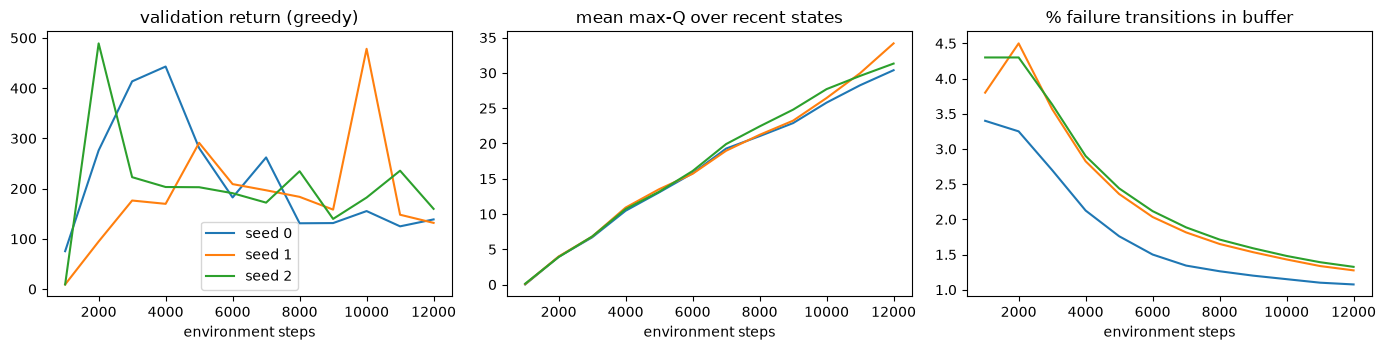
\includegraphics[width=\linewidth]{fig_n0_diagnosis.png}
\end{block}

\column{0.5\textwidth}
\begin{block}{N1: choosing the recipe (dev seeds)}
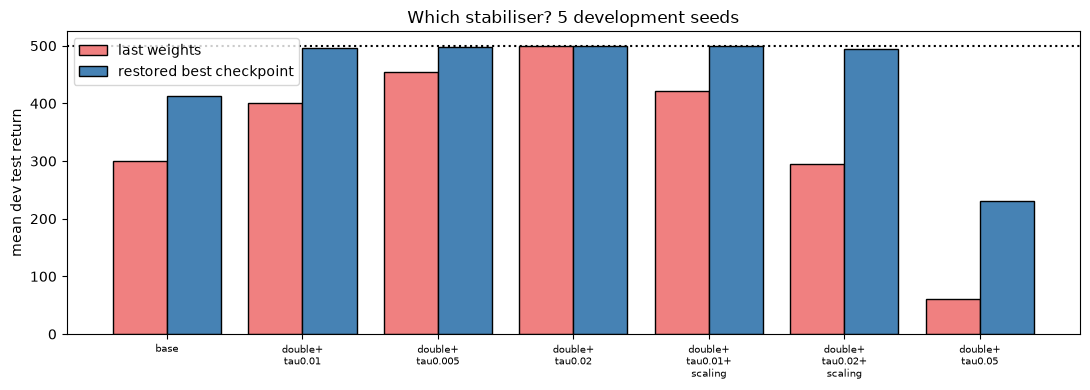
\includegraphics[width=\linewidth]{fig_n1_recipe_dev.png}
\end{block}

\end{columns}
\end{frame}

% =========================================================
\section{Conclusion and Resources}

\begin{frame}{Conclusion}
\begin{itemize}
  \item \textbf{OG}: two variables and a switching rule are enough ($K\le0.5$ reaches 500); angle-only fails by pole, angular-velocity-only fails by cart.
  \item \textbf{NN}: a ReLU Q-network gets close to the rule (480.3 vs 491.7) only with stabilisers, and the biggest single factor is \alert{restoring the best checkpoint}; patience saves steps only with a grace period.
  \item \textbf{CPU vs GPU}: for this network the CPU wins (GPU 2.3$\times$ slower); the GPU pays off only for large models or batches.
  \item \textbf{Nuclei}: parallel runs give identical results; speed-up is real but sub-linear.
  \item \textbf{Main limitation}: small samples (5 seeds), selection on seen seeds, trimmed timing runs.
  \item \textbf{Future work}: more seeds, a clean 1-core time for every arm, profile where update time goes, train with wide start noise.
\end{itemize}
\end{frame}

\begin{frame}{Ideas to improve the CartPole activity}
\small
\begin{itemize}
  \item \textbf{Fix OG}: human-play text vs output; implement \texttt{policy\_mine} and tune $K$; make Experiment A measure over episodes; make Experiment C a real ablation.
  \item \textbf{Count failure modes} (pole / cart / time) in \texttt{evaluate\_policy}: it turns a number into an explanation.
  \item \textbf{Separate tuning seeds from test seeds}; report per seed, not only mean $\pm$ std (returns are capped at 500).
  \item \textbf{NN}: validate on greedy return; always restore the best weights; give patience a grace period; test the neighbours of a tuned setting ($\tau$).
  \item \textbf{Hardware}: small networks on CPU; show the batch/width sweep so the GPU break-even is visible.
  \item \textbf{Nuclei}: size \texttt{n\_jobs} to physical cores; keep seeding inside the worker; check identical results.
  \item \textbf{Time}: record it for every experiment (a ledger of every cell is in the notebook).
\end{itemize}
\end{frame}

\begin{frame}{Resources}
\begin{itemize}
  \item Combined notebook:
  \texttt{rl101-cartpole-OG-vs-NN-vs-Nuclei.ipynb}

  \vspace{0.3cm}

  \item Sources kept untouched:
  \texttt{rl101-cartpole-basis-activity.ipynb}, \texttt{rl101-DQN\_Replay\_TargetNet\_Bryan.ipynb}

  \vspace{0.3cm}

  \item Written analysis: \texttt{CARTPOLE\_PROJECT\_STATUS\_AND\_IMPLEMENTATION\_ANALYSIS.txt}

  \vspace{0.3cm}

  \item Reading: M.~Hu, \emph{The Art of Reinforcement Learning}, Apress 2023; Gymnasium CartPole-v1 documentation.
\end{itemize}
\end{frame}

\begin{frame}{Backup: likely questions}
\scriptsize
\begin{itemize}
  \item \textbf{Why does angle $+K\cdot$angular velocity work?} PD / sliding-mode: on $s=0$ the angle decays as $e^{-t/K}$; angle alone has no damping, velocity alone ignores tilt (cart drifts).
  \item \textbf{Why is patience on return, not loss?} The loss keeps changing with the target scale while the greedy return swings between 100 and 500; the return is the goal.
  \item \textbf{Patience or checkpoint restore, which helped?} Restore: plain 148 $\to$ 367. Patience (with grace) then saved 19\% of the steps at equal quality.
  \item \textbf{Is the recipe proven better?} Only weakly: $+113$ on 5 fresh seeds; the development gap was inflated by selection.
  \item \textbf{Why is the GPU slower?} The environment is on the CPU: each step pays a round trip and a copy; 17,410 parameters do too little work to repay it.
  \item \textbf{Do more cores change results?} No: identical curves at 1, 2, 4, 8 workers; only time changes.
\end{itemize}
\end{frame}

\begin{frame}{Q \& A}
\centering
\Large Questions?
\end{frame}

\end{document}
